
\chapter{Kraftar}

\begin{comment}
\begin{quote}
    \textit{\duck{No prediction whatsoever can be made from a definition. One might sit in an armchair all day long and define words at will, but to find out what happens when two balls push against each other, or when a weight is hung on a spring, is another matter altogether, because the way the bodies behave is something completely outside any choice of definitions.}}
    \begin{flushright}
    - Richard Feynman
    \end{flushright}
\end{quote}
\end{comment}


\section{Útdráttur úr Principia eftir Newton}

\subsection*{AXIOMS, OR THE LAWS OF MOTION}

\begin{enumerate}[label = \textbf{Law \arabic*} \hspace{0.3cm}]
    \item \textit{Every body perseveres in its state of being at rest or of moving uniformly straight forward, except insofar as it is compelled to change its state by forces impressed.}
    \vspace{0.25cm}
    
    \hspace{0.3cm} Projectiles persevere in their motions, except insofar as they are retarded by the resistance of the air and are impelled downward by the force of gravity. A spinning hoop, which has parts that by their cohesion continually draw one anohter back from rectilinear motions, does not cease to rotate, except insofar as it is retarded by the air. And larger bodies - planets and comets - preserve for a longer time both their progressive and their circular motions, which take place in spaces having less resistance.
    \item \textit{A change in motion is proportional to the motive force impressed and takes place along the straight line in which that force is impressed.} 
     \vspace{0.25cm}
    
    \hspace{0.3cm} If some force generates any motion, twice the force will generate twice the motion, and three times the force wil generate three times the motion, whether the force is impressed all at once or successively by degrees. And if the body was previously moving, the new motion (since motion is always in the same direction as the generative force) is added to the original motion if that motion was in the same direction or is subtracted from the original motion if it was in the opposite direction or, if it was in an oblique direction, is combined obliquely and compounded with it according to the directions of both motions.
    \item \textit{To any action there is always an opposite and equal reaction; in other words, the actions of two bodies upon each other are always equal and always opposite in direction.}
     \vspace{0.25cm}
    
    \hspace{0.3cm} Whatever presses or draws something else is pressed or drawn just as much by it. If anyone presses a stone with a finger, the finger is also pressed by the stone. If a horse draws a stone tied to a rope, the horse will (so to speak) also be drawn back equally toward the stone, for the rope, stretched out at both ends, will urge the horse toward the horse by one and the same endeavor to go slack and will impede the forward motion of the one as much as it promotes the forward motion of the other. If some body impinging upon another body changes the motion of that body in any way by its own force, then, by the force of the other body (because of the equality of their mutual pressure), it also will in turn undergo the same change in its own motion in the opposite direction. By means of these actions, equal changes occur in the motions, not in the velocities - that is, of course, if the bodies are not impeded by anything else. For the changes in velocities that likewise occur in opposite directions are inversely proportional to the bodies because the motions are changed equally. This law is valid also for attractions, as will be proved in the next scholium.
\end{enumerate}

\newpage

\section{Lögmál Newtons}

\begin{quote}
    \textit{\duck{No prediction whatsoever can be made from a definition. One might sit in an armchair all day long and define words at will, but to find out what happens when two balls push against each other, or when a weight is hung on a spring, is another matter altogether, because the way the bodies behave is something completely outside any choice of definitions.}}
    \begin{flushright}
    - Richard Feynman
    \end{flushright}
\end{quote}

Við skulum nú loksins fjalla um kraftahugtakið. Það er afskaplega öflugt en á sama tíma mjög einfalt:

\begin{tcolorbox}
\begin{definition}
Lítum á hlut með massa $m$ sem verður fyrir hröðun $a$. \textbf{Heildarkrafturinn} sem verkar á hlutinn er þá gefinn með:
\begin{align*}
    F_{\text{heild}} = ma.
\end{align*}
\end{definition}
\end{tcolorbox}

Við skrifum stundum til einföldunar $F = ma$. Við segjum síðan að hröðunin sem að hlutur verður fyrir sé vegna kraftsins sem verkar á hlutinn. En það er í rauninni hringskilgreining því við segjum að krafturinn sé vegna hröðunarinnar sem að hluturinn finnur fyrir. Við athugum að einingarnar á krafti eru gefnar með $[F] = [ma] = [m][a] = \si{kg.m/s^2}$.
Þessi stærð hefur fengið nafnið Newton og er táknuð með $\si{N} = \si{kg.m/s^2}$. Lögmál Newtons eru í íslenskri þýðingu eftirfarandi:

\begin{tcolorbox}[left=1.8cm]
\begin{enumerate}[label = \textbf{Lögmál \arabic*} \hspace{0.25cm}]
    \item \textit{Sérhver hlutur heldur áfram að vera í kyrrstöðu, eða á jafnri hreyfingu eftir beinni línu, nema kraftar sem á hann verka þvingi hann til að breyta því ástandi.}
    
    \item \textit{Breyting hreyfingarinnar er í réttu hlutfalli við hreyfikraftinn sem verkar; og hún verður í stefnu beinu línunnar sem krafturinn verkar eftir.} 
    
    \item \textit{Gagnstætt sérhverju átaki er ávallt jafnstórt gagntak, eða gagnkvæmar verkanir tveggja hluta hvors á annan eru ávallt jafnstórar og í gagnstæða stefnu.}
\end{enumerate}
\end{tcolorbox}
\subsection*{Fyrsta lögmálið}

Fyrsta lögmálið, sem gjarnan er nefnt tregðulögmálið, segir okkur að eina leiðin til þess að breyta hraða hlutar sé með því að beita einhverjum heildarkrafti $F$ á hann. En $F = ma$ svo það er jafngilt því að hann verði fyrir hröðun $a$. En fyrir fasta hröðun $a = 0$ gildir að $v = v_0 + at = v_0 = \text{fasti}$. Við höfum því að:
\begin{center}
\begin{tcbox}[nobeforeafter]{$F = 0 \iff a = 0 \iff v = \text{fasti}.$}
\end{tcbox}
\end{center}


\subsection*{Annað lögmálið}

Annað lögmálið segir okkur að hreyfing hlutar er vegna hröðunarinnar sem hluturinn verður fyrir vegna samanlagðra krafta sem verka á hlutinn. Ef $F_1, F_2, \ldots, F_n$ eru kraftar sem verka á hlut þá ritum við oft
\begin{center}
\begin{tcbox}[nobeforeafter]{$F_{\text{heild}} = F_1 + F_2 + \ldots + F_n.$}
\end{tcbox}
\end{center}

\subsection*{Þriðja lögmálið}

Loks segir þriðja lögmálið okkur að ef hlutur $A$ verkar með krafti $F_A$ á hlut $B$ þá verkar hlutur $B$ með jafnstórum gagnverkandi krafti á hlut $A$, þ.e.a.s.
\begin{center}
\begin{tcbox}[nobeforeafter]{$F_A = -F_B.$}
\end{tcbox}
\end{center}

\section{Nokkrir kraftar}

\subsection*{Þyngdarkraftur}

Fyrsti krafturinn sem við nefnum er kannski sá sem flestir þekkja:

\begin{tcolorbox}
\begin{definition}
    Lítum á hlut með massa $m$ sem er staddur í þyngdarsviði með þyngdarhröðun $g$. Þá verkar á hann kraftur
    \begin{align*}
        F_g = mg,
    \end{align*}
    beint niður í áttina að jörðinni, sem kallast \textbf{þyngdarkraftur}.
\end{definition}
\end{tcolorbox}

\begin{figure}[H]
    \centering
    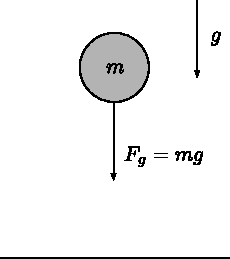
\includegraphics{figures/mg.pdf}
    \caption{Hlutur með massa $m$ í þyngdarsviði með þyngdarhröðun $g$ finnur fyrir þyngdarkrafti $F_g = mg$.}
    \label{fig:stoduorka}
\end{figure}

\subsection*{Þverkraftur}

Ef við stöndum kyrr á jörðinni, þá er heildarkrafturinn á okkur núll (því við erum ekki á hreyfingu svo hröðun okkar er núll og því er heildarkrafturinn það líka samkvæmt fyrsta lögmáli Newtons). En þyngdarkrafturinn verkar alltaf á okkur svo að það hlítur að vera jafn stór kraftur sem verkar í öfuga stefnu miðað við þyngdarkraftinn sem heldur okkur kyrrum. Sá kraftur nefnist þverkraftur og er táknaður með $\text{Þ}$. Þverkrafturinn verkar alltaf hornrrétt frá yfirborði flatarins á hlutinn sem hvílir á fletinum. 

\begin{figure}[H]
    \centering
    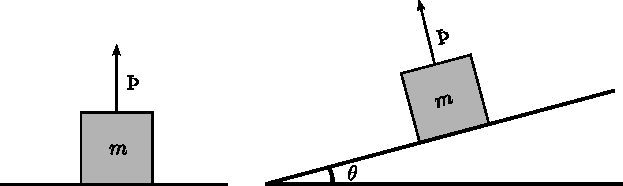
\includegraphics{figures/thverkraftur.pdf}
    \caption{Hlutur sem hvílir ofan á öðrum fleti finnur fyrir þverkrafti, $\text{Þ}$, frá fletinum, hornrétt á yfirborðið.}
    \label{fig:normalforce}
\end{figure}

Á mynd \ref{fig:normalforce} sjáum við hvernig þverkrafturinn, $Þ$, sem verkar á hlut, breytist eftir því sem að við höllum fletinum sem hann hvílir á um horn $\theta$ miðað við lárétt. Á myndinni vinstra megin höfum við að $Þ = mg$ en hinsvegar á hægri myndinni höfum við að $Þ = mg\cos\theta$. \\

\textbf{Varúð:} Einföld sál gæti haldið að þverkrafturinn og þyngdarkrafturinn væru þriðja lögmáls par. Það er hinsvegar ekki rétt! Því þegar við stöndum á jörðinni þá verkum við með krafti á jörðina sem ýtir henni niður. Jörðin ýtir þá til baka á okkur með jafn stórum gagnverkandi krafti. Sá kraftur er þverkrafturinn. Það er mikilvægt að átta sig á því að kraftarnir sem um ræðir í þriðja lögmáli Newtons verka alltaf á sitt hvorn hlutinn. Því geta þyngdarkrafturinn og þverkrafturinn ekki verið þriðja lögmáls par.

\subsection*{Núningskraftur}

Á milli sérhverra tveggja yfirborða verkar núningskraftur sem er háður efnunum sem snertast. Við lýsum stærð núningskraftsins milli tveggja efna með \textbf{núningsstuðlinum}, $\mu$. Því lægri sem núningsstuðullinn er því minni núningurinn sem verkar á milli yfirborðanna. Til dæmis er núningsstuðullinn milli ís og ís frekar lágur ($\mu = \SI{0.02}{}$) en milli málms og viðar hár ($\mu = \SI{0.5}{}$). Þið hafið eflaust tekið eftir því að  að okkur hefur tekist að ýta hlut af stað þá er auðveldara að draga hann meðfram öðru yfirborði. Þetta er vegna þess að við höfum í rauninni tvær mismunandi gerðir af núningsstuðlum. Annars vegar hreyfinúningsstuðullinn, $\mu_k$ sem lýsir núningskraftinum á milli tveggja hluta sem eru á hreyfingu miðað við hvorn annann og hinsvegar kyrrstöðunúningsstuðullinn $\mu_s$ sem lýsir núningskraftinum á milli tveggja hluta sem eru kyrrir miðað við hvorn annan. Athugið að kyrrstöðunúningsstuðullinn er alltaf stærri en hreyfinúningsstuðullinn því eftir að við höfum komið hlut af stað er auðveldara að draga hann áfram. Við höfum almennt að núningskraftinn má reikna með eftirfarandi lögmáli:
\begin{tcolorbox}
\begin{theorem}
Lítum á hlut sem er dreginn meðfram yfirborði. Látum núningsstuðulinn milli hlutarins og flatarins vera $\mu$. Látum $\text{Þ}$ vera þverkraftinn sem flöturinn verkar með á hlutinn og látum $F_{\text{nún}}$ vera núningskraftinn milli flatarins og hlutarins. Þá gildir að:
\begin{align*}
    F_{\text{nún}} = \mu \text{Þ}.
\end{align*}
Stefna kraftsins er gagnstæð hreyfingu hlutarins miðað við flötinn.
\end{theorem}
\end{tcolorbox}

\begin{figure}[H]
    \centering
    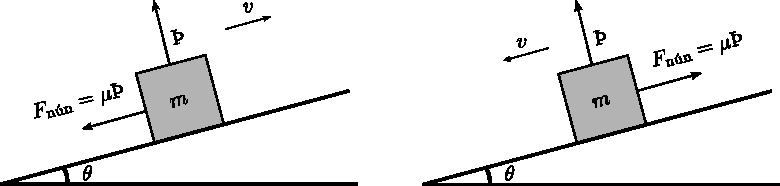
\includegraphics{figures/nun.pdf}
    \caption{Hlutur sem nuddast upp við annan flöt finnur fyrir núningskrafti gagnstætt hreyfingunni.}
    \label{fig:fnun}
\end{figure}

\textbf{Athugið:} Hugsum okkur að hluturinn sé kyrr (þ.e.~ekki á hreyfingu miðað við yfirborðið sem hann hvílir á). Ef við beitum krafti $F \leq \mu Þ$ á hlutinn þá mun hann haldast kyrr því krafturinn $F$ er ekki nógu stór til þess að yfirvinna núningskraftinn. Í því tilviki er núningskrafturinn jafn stór og krafturinn $F$, þ.e. $F_{\text{nún}} = F$ til að halda hlutnum kyrrum. Við ættum því tæknilega séð að skrifa $F_{\text{nún}} \leq \mu Þ$ til að gefa þetta til kynna.


\subsection*{Togkraftur}

Þegar við togum í reipi þá togar reipið til baka í okkur með jafn stórum gagnverkandi krafti samkvæmt þriðja lögmáli Newtons. Þessi kraftur nefnist \textbf{togkraftur}.

\begin{figure}[H]
    \centering
    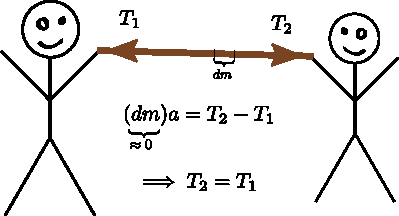
\includegraphics{figures/togkraftur.pdf}
    \caption{Togkrafturinn í reipinu er sá sami alls staðar að því gefnu að reipið sé svo gott sem massalaust.}
    \label{fig:togkraftur}
\end{figure}


\section{Fleiri kraftar}

\subsection*{Gormkraftur}

Hugsum okkur gorm. Ef við drögum hann frá jafnvægisstöðunni sinni og sleppum honum þá skýst hann til baka í átt að jafnvægisstöðunni. Því meira sem við drögum því erfiðara er að halda honum og ef við missum tak á honum þá skýst hann þeim mun meira af stað. Þessu fyrirbæri má lýsa með eftirfarandi lögmáli:
\begin{tcolorbox}
\begin{definition}
Lítum á gorm með gormstuðul $k$ sem er í fjarlægð $x$ frá jafnvægisstöðu sinni. Þá er \textbf{gormkrafturinn}, $F_k$, sem verkar á gorminn gefinn með:
\begin{align*}
    F_k = -kx.
\end{align*}
\end{definition}
\end{tcolorbox}
Gormstuðullinn, $k$, getur verið háður efninu sem gormurinn er gerður úr, lögun gormsins og stærð hans. Við skulum skoða hvaða einingar gormstuðullinn hefur. Nú er $\left[ F \right] = \si{N}$ og $\left[x \right] = \si{m}$ svo að $\left[ k \right] = \left[F\right]/ \left[ x \right] = \si{N/m}$.

\begin{figure}[H]
    \centering
    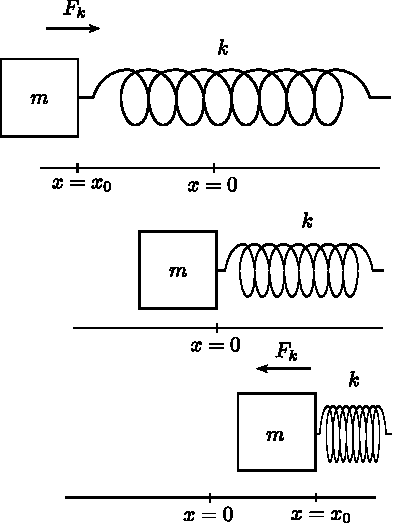
\includegraphics{figures/gormur.pdf}
    \caption{Gormkrafturinn er háður gormstuðli gormsins og fjarlægð gormsins frá jafnvægisstöðunni.}
    \label{fig:gormur.pdf}
\end{figure}

\subsection*{Loftmótsstaða}

Venjulega hunsum við loftmótstöðu í dæmunum sem við reiknum, en núna skulum við gera henni góð skil (svo að við getum hunsað hana aftur með góðri samvisku). Loftmótstaðan sem verkar á hlutinn er háð þverskurðarflatarmálinu, $A$, eðlismassa loftsins, $\rho$, og hraða hlutarins $v$. Með víddargreiningu sjáum við að:
\begin{align*}
    [\rho A v^2] = (\si{kg/m^3}) (\si{m^2}) (\si{m/s})^2 = \si{kg.m/s^2} = \si{N}.
\end{align*}
Við höfum þá með víddargreiningu að til sé fasti $\alpha$ þannig að loftmótstöðukrafturinn, $F_L$ sé gefinn með:
\begin{align*}
    F_L = \alpha \rho A v^2.
\end{align*}
Við höfum þar að auki að í einföldum aðstæðum er $\rho_{\text{loft}} = \text{fasti}$ og $A = \text{fasti}$. Við ályktum því að rita megi:
\begin{center}
\begin{tcbox}[nobeforeafter]{$F_L = \beta v^2.$}
\end{tcbox}
\end{center}
Þar sem $\beta = \alpha \rho A$ er fasti með einingar $[\beta] = \si{kg/m}$ og er háður eðlismassa lofts og þverskurðarflatarmálinu.


\begin{comment}
\subsection*{Rafkraftur}

Árið 1785 setti Charles-Augustin de Coulomb fram eftirfarandi lögmál um rafkraftinn milli tveggja hlaðinna agna með hleðslu $q_1$ og $q_2$ í fjarlægð $r$ frá hvorri annarri:
\begin{align*}
F_e = k\frac{q_1q_2}{r^2}
\end{align*}
þar sem $k = \SI{8.99e9}{N m^2/C^2}$ er fasti sem nefnist fasti Coulombs. Rafeindin hefur hleðslu $-e = \SI{-1.602e-19}{C}$ og massa $m_e = \SI{9.11e-31}{kg}$ á meðan róteindin hefur hleðslu $+e = \SI{1.602e-19}{C}$ og massa $m_p = \SI{1.67e-27}{kg}$.
\end{comment}



\section{Sýnidæmi}

\subsection*{Skábrettadæmi}

Skoðum kassa með massa $m$ sem hvílir á skábretti sem hallar um $\theta$ gráður miðað við lárétt. Gerum ráð fyrir að núningsstuðullinn milli kassans og skábrettisins sé $\mu$. Þá verka eftirfarandi kraftar á kassann: Þyngdarkrafturinn, $F_g$, þverkrafturinn, $\text{Þ}$ og núningskrafturinn, $F_{\text{nún}}$. Ef hornið $\theta$ er nógu lítið þá mun þyngdarkraftinum ekki takast að yfirvinna núningskraftinn og kassinn mun haldast kyrr. Því er til minnsta horn, $\theta_{\text{min}}$, þannig að fyrir $\theta \leq \theta_{\text{min}}$ rennur kassinn ekki niður skábrettið en fyrir $\theta > \theta_{\text{min}}$ rennur kassinn niður skábrettið. Hlutir sem eru ekki á hreyfingu eru óspennandi svo við skoðum tilvikið þegar $\theta > \theta_{\text{min}}$.

\begin{figure}[H]
    \centering
    \begin{tikzpicture}[scale=2.5]
    
          %  Hjálparlínur
         % \draw[help lines] (-1,-1) grid (7,3);
        
          %  Skilgreiningar á hnitum
        \coordinate (A) at (0, 0);
        \coordinate (B) at (4,0);
        \coordinate (C) at (4,1.8);
        \coordinate (fer1) at (2.29284, 1.02846);
        \coordinate (fer2) at (2.80037, 1.26);
        \coordinate (fer3) at (2.59199, 1.77105);
        \coordinate (fer4) at (2.07716, 1.53591);
        \coordinate (theta) at (0.95,0.22);
        \coordinate (m) at (2.44101, 1.39482);
        \coordinate (mtoppur) at (2.35, 1.67);
        \coordinate (th) at (2.18, 2.1);
        \coordinate (mbotn) at (2.55, 1.15);
        \coordinate (fg) at (2.55, 0.3);
        \coordinate (fglidun) at (2.84, 0.46);
        \coordinate (mhhlid) at (2.7, 1.5);
        \coordinate (fnun) at (3.4, 1.83);
        
        
          %  Einföldustu teikningar
        \draw[line width = 1] (A) -- (B) -- (C) -- (A); %Þríhyrningur
        \draw[line width = 1] (fer1) -- (fer2) -- (fer3) -- (fer4) -- (fer1); %Massi
        \draw[->] (mtoppur) -- (th);
        \draw[->] (mbotn) -- (fg);
        \draw[->] (mhhlid) -- (fnun);
         \draw[dotted] (mbotn) -- (fglidun) -- (fg);

          %  Nokkrar merkingar
        \draw[line width = 1] (0.8, 0) arc [radius=0.8, start angle=0, delta angle=24.23];
        \draw[line width = 0.5] (2.55, 0.9) arc [radius=0.25, start angle=270, delta angle=24.23];
        \node at (theta) {\Large \(\theta\)};
        \node at (2.35,0.6) { \(F_g\)};
        \node[rotate=10] at (2.63,0.78) { \(\theta\)};
        \node[rotate=24.23] at (m) {\Large \(m\)};
        \node[rotate=20] at (2.15,1.8) { \(\text{Þ}\)};
        \node[rotate=20] at (3,1.8) { \(F_{\text{nún}}=\mu \text{Þ}\)};
        \node[rotate=24] at (2.75,0.25) {\small \(F_{g}\sin\theta\)};
        \node[rotate=-66] at (2.8,0.85) {\small \(F_{g}\cos\theta\)};
    \end{tikzpicture}
\end{figure} 

\textbf{Dæmi:} Ákvarðið hröðun kassans, $a$, niður samsíða skábrettinu að því gefnu að $\theta > \theta_{\text{min}}$. \\

\textbf{Lausn:} Við veljum hnitakerfið þannig að $x$-ásinn sé samsíða skáplaninu (í stefnu niður) og $y$-ásinn þvert á $x$-ásinn upp. Samkvæmt öðru lögmáli Newtons er heildarkrafturinn sem verkar á kassann þá summa allra kraftanna sem verka á kassann. Kraftarnir sem verka á kassann eru þyngdarkrafturinn, þverkrafturinn og núningskrafturinn. Við vitum að heildarhröðunin í $y$-stefnuna verður núll því massinn er að renna á skáplaninu án þess að losna frá því. Við höfum því að:
\begin{align*}
    m \begin{pmatrix}
    a \\
    0
    \end{pmatrix} = \vec{F}_{\text{heild}} =  \vec{F}_g + \vec{F}_{\text{nún}} + \vec{Þ} = \begin{pmatrix}
    mg\sin\theta \\
    -mg\cos\theta
    \end{pmatrix} + \begin{pmatrix}
    -\mu Þ \\
    0
    \end{pmatrix} + \begin{pmatrix}
    0 \\
    Þ
    \end{pmatrix}.
\end{align*}
Við sjáum þá af neðri jöfnunni að:
\begin{align*}
    0 = -mg\cos\theta + Þ \implies Þ = mg\cos\theta,
\end{align*}
en þá verður efri jafnan:
\begin{align*}
    ma = mg\sin\theta - \mu Þ = mg\sin\theta - \mu mg\cos\theta
\end{align*}
styttum út $m$ og tökum $g$ út fyrir sviga og höfum þá:
\begin{center}
\begin{tcbox}[nobeforeafter]{$a = g\left( \sin\theta - \mu \cos\theta \right).$}
\end{tcbox}
\end{center}

\begin{comment}
Við skulum skoða jöfnu (\ref{eq:skabretti}) nánar.
Ef $\theta = \ang{90}$ væri skábrettið lóðrétt og kubburinn myndi falla niður með þyngdarhröðuninni $g$.
Svo við myndum búast við að $a = g$. En ef við stingum inn $\theta = \ang{90}$ þá fáum við einmitt að $a = g$ (því $\cos(\ang{90})  = 0$).
Þetta bendir til þess að við höfum gert eitthvað rétt í útleiðslunni!
\end{comment}

\textbf{Dæmi:} Ákvarðið minnsta hornið, $\theta_{\text{min}}$, þannig að kassinn renni niður skábrettið. \\

\textbf{Lausn:} Ef $\theta > \theta_{\text{min}}$ þá er $a > 0$ en þegar $\theta = \theta_{\text{min}}$ þá er $a = 0$ og kassinn rennur niður skábrettið með jöfnum hraða. Við fáum því að $0 = g(\sin\theta - \mu \cos\theta)$ en það gefur okkur að $\sin\theta = \mu \cos\theta$ sem er jafngilt því að $\mu = \frac{\sin\theta}{\cos\theta} = \tan\theta$. Þetta gildir aðeins fyrir hornið $\theta = \theta_{\text{min}}$ svo við höfum sýnt að $\mu = \tan(\theta_{\text{min}})$.

\begin{comment}
\begin{center}
\begin{tcbox}[nobeforeafter]{$\mu = \tan(\theta_{\text{min}}).$}
\end{tcbox}
\end{center}
Þessa niðurstöðu má nota til þess að finna núningsstuðulinn milli tveggja efna með því að láta kubb renna niður skábretti með jöfnum hraða. Við getum líka snúið þessu við þannig að $\theta_{\text{min}} = \arctan(\mu)$.
\end{comment}

\textbf{Dæmi:} Ákvarðið hraða kassans þegar hann hefur runnið niður skábrettið úr hæð $h$. \\

\textbf{Lausn:} Ef við byrjum á því að hunsa núninginn þá fáum við einfaldlega með orkuvarðveislu að:
\begin{align*}
    \frac{1}{2}mv^2 = mgh \implies v_{\text{orka}} = \sqrt{2gh}.
\end{align*}
Við skoðum núna hvað gerist þegar hluturinn verður fyrir núningskrafti á leiðnni niður. Ef kubburinn byrjar í hæð $h$ þá er lengdin sem hann á eftir að renna niður skábrettið $\Delta s = \frac{h}{\sin\theta}$. Við vitum að hröðun kassans niður skábrettið er gefin með $a = g(\sin\theta - \mu \cos\theta)$. Við fáum því með tímaóháðu jöfnunni að:
\begin{align*}
    2a \Delta s = v^2 - v_0^2 \implies v = \sqrt{2a\Delta s} = \sqrt{2g(\sin\theta - \mu \cos\theta)\frac{h}{\sin\theta}} = \sqrt{2gh\left(1-\mu\cot\theta \right)}
\end{align*}
Við getum þannig fundið hversu mikil orka, $W_{\text{nún}}$, tapaðist í núning á leiðinni niður:
\begin{align*}
    W_{\text{nún}} = \Delta K = \frac{1}{2}m {v_{\text{orka}}}^2 - \frac{1}{2}mv^2 = mgh - mgh(1-\mu \cot\theta) = \mu \cot\theta \, mgh.
\end{align*}

\subsection*{Togkraftadæmi}

Lítum á tvo massa $m_A$ og $m_B$ sem tengdir eru saman með reipi. Látum Matta verka á massa $m_A$ með krafti $F_M$ yfir horninu $\theta$ miðað við lárétt. Hver er hröðun massans $m_A$? Hver er hröðun massans $m_B$? Hver er togkrafturinn í reipinu á meðan Matti verkar á massann $m_A$?

\begin{figure}[H]
    \centering
    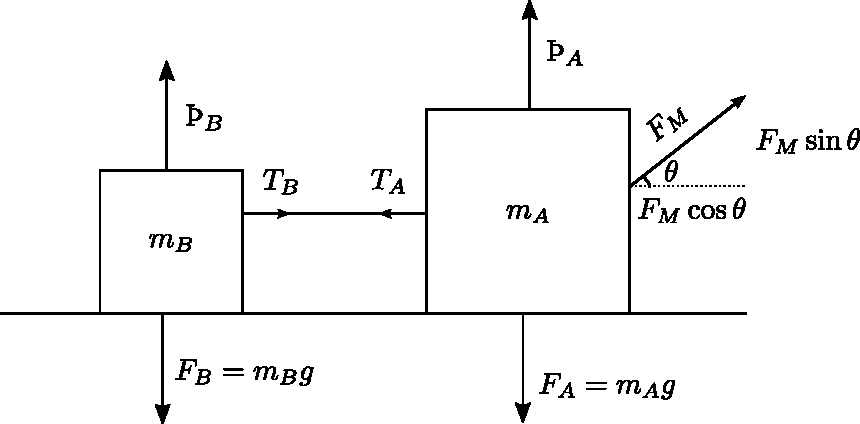
\includegraphics[scale = 0.7]{figures/ytakubb.pdf}
\end{figure}

\textbf{Lausn:} Við stillum upp kraftajöfnum fyrir báða kassana. Hröðun kassans $m_A$ er jöfn hröðun kassans $m_B$. Á kassa $A$ verka kraftarnir $F_M, F_g, Þ$ og $T$. Við höfum þá (að því gefnu að $F_M$ sé ekki nógu stór til þess að lyfta kassa $A$) að:
\begin{align*}
    m_A\begin{pmatrix}
    a \\
    0
    \end{pmatrix} = \begin{pmatrix}
    F_M \cos\theta - T_A \\
    F_M\sin\theta + Þ_A - F_A
    \end{pmatrix}
\end{align*}
Hinsvegar höfum við fyrir massa $B$ að kraftajafnan verður:
\begin{align*}
   m_B \begin{pmatrix}
a \\ 0
\end{pmatrix} = \begin{pmatrix}
T_B \\ Þ_B - F_B
\end{pmatrix} 
\end{align*}
Leggjum saman báðar efri jöfnurnar og notum að $T_A = T_B$ og fáum þá að:
\begin{align*}
    \left(m_A + m_B \right)a = F_M \cos\theta
\end{align*}
svo við ályktum að $a = \frac{F_M \cos\theta}{m_A + m_B}$. Til þess að finna togkraftinn í reipinu þá fáum við að:
\begin{align*}
    T = T_B = m_Ba = \frac{m_B}{m_A + m_B}F_M \cos\theta.
\end{align*}

\subsection*{Trissudæmi}

Látum tvo kassa, $1$ og $2$ með massa $m_1$ og $m_2$ vera tengda saman með bandi. Kassi $1$ hangir í frjálsu falli yfir núningslausri trissu en kassi $2$ liggur á borði. Finnið hröðun kerfisins ef núningsstuðullinn milli borðsins og kassa 2 er $\mu$. Finnið togkraftinn í bandinu.

\begin{figure}[H]
    \centering
    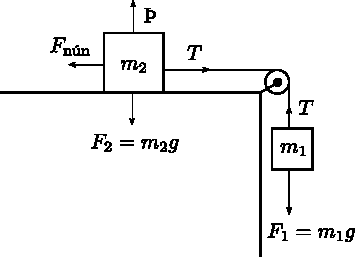
\includegraphics{figures/trissudaemi.pdf}
\end{figure}

Við stillum upp kraftajöfnum fyrir massana tvo. Höfum fyrir kassa $1$ að (veljum stefnu í átt niður að gólfinu)
\begin{align*} 
F_{\text{heild}} = m_1a = m_1g - T
\end{align*}
en fyrir kassa $2$ höfum við eftirfarandi kraftajöfnu:
\begin{align*}
    F_{\text{heild}} = m_2a = T - F_{\text{nún}} = T - \mu m_2 g
\end{align*}
Leggjum saman jöfnurnar og fáum þá að:
\begin{align*}
    (m_1 + m_2)a = m_1g - \mu m_2 g
\end{align*}
svo við fáum að
\begin{align*}
    a = \frac{m_1-\mu m_2}{m_1 + m_2}g
\end{align*}
En þá getum við fundið togkraftinn með því að athuga að
\begin{align*}
    T = -m_1(a-g) = -m_1 g \left( \frac{m_1-\mu m_2}{m_1 + m_2} - 1 \right) = -m_1 g \left( \frac{m_1 - \mu m_2 - \left( m_1 + m_2 \right)}{m_1 + m_2} \right) = \frac{(\mu +1)m_1 m_2}{m_1 + m_2}g
\end{align*}

\subsection*{Lyftudæmi}

Ónefndur nemandi í 5.XY ætlar að reyna að sleppa við það að þurfa að fara í lyftuna í Cösu Nova. Til þess að sleppa við það ætlar nemandinn að beita hugviti sínu til þess að giska á niðurstöðurnar sem að vondi, strangi kennarinn hans (nefnum engin nöfn) ætlar að spurja hann út úr. Hann stillir því upp kraftajöfnunum sem að verka á lyftuna og nemandann sem stendur á voginni. Látum lyftuna hafa massa $M_L$ og látum ónefnda nemandann hafa massa $m_n$. Ef lyftan er á leiðinni upp er $a > 0$ (miðað við stefnu skilgreinda upp) og kraftajafnan verður fyrir lyftuna:
\begin{align*}
    m_L a = F_{\text{lyfta}} - M_L g
\end{align*}
en hinsvegar fyrir ónefnda nemandan verður jafnan
\begin{align*}
    m_n a = Þ - m_n g
\end{align*}
en þar sem að $a > 0$ þá fáum við að $Þ > m_n g$ svo að þyngd nemandans virðist aukast (samkvæmt voginni) þegar hann fer upp. En hinsvegar ef við erum á leiðinni niður þá verður kraftajafnan fyrir ónefnda nemandann (með $a > 0$ og stefnuna skilgreinda niður)
\begin{align*}
    m_n a = m_n g - Þ
\end{align*}
og ef $a > 0$ þá er $m_ng - Þ > 0$ svo við ályktum að þyngd nemandans virðist minnka á leiðinni niður. Hinsvegar á miðkaflanum þá ferðast lyftan með jöfnum hraða og þá höfum við $a = 0$ og $Þ = m_ng$ og þyngd nemandans á voginni virðist vera sú sama.

\newpage

\subsection*{Vél Atwoods}

\begin{figure}[H]
    \centering
    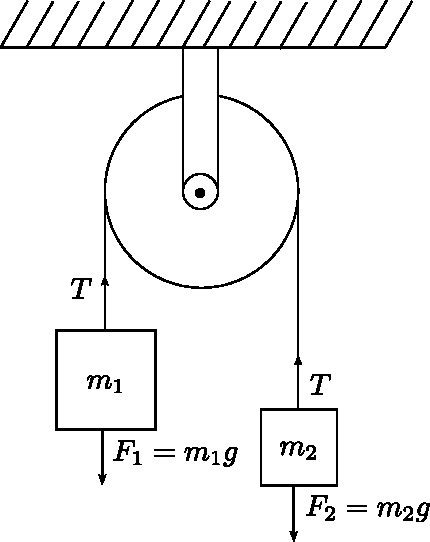
\includegraphics[scale = 0.7]{figures/atwood.pdf}
\end{figure}

Ef við gerum ráð fyrir að $m_1 > m_2$ þá þykir okkur eðlilegt að þyngri massinn byrji að fara niður með hröðun $a$ en sá léttari færist upp með hröðun $a$. Finna á hröðunina $a$ og togkraftinn í strengnum. \\

\textbf{Lausn:} Við stillum upp kraftajöfnum fyrir massana:
\begin{align*}
    m_1 a = m_1 g - T
\end{align*}
og
\begin{align*}
    m_2 a = T - m_2 g
\end{align*}

svo við höfum þá að
\begin{align*}
    (m_1 + m_2)a = (m_1 - m_2)g
\end{align*}
sem gefur því að 
\begin{align*}
    a = \frac{m_1 - m_2}{m_1 + m_2}
\end{align*}
en þar með höfum við að togkrafturinn sé
\begin{align*}
    T = m_1 (g-a) = m_1 g \left( 1-  \frac{m_1 - m_2}{m_1 + m_2} \right) = m_1 g \left( \frac{m_1 + m_2 - (m_1 - m_2)}{m_1 + m_2} \right) = \left(\frac{2m_1 m_2}{m_1 + m_2}\right) g
\end{align*}

Víddargreining getur líka verið gott tól til þess að meta hvort að svarið sem að við höfum fundið standist nánari athuganir. Til dæmis fengum við að hröðun massanna í vél Atwoods væri (ef $m_1 > m_2$)
\begin{align*}
    a = \frac{m_1 - m_2}{m_1 + m_2}g
\end{align*}
við getum athugað hverjar víddirnar eru beggja meginn jafnaðarmerkisins (þá eru oft settir hornklofar í kringum stærðina) þannig við höfum að:
\begin{align*}
   \explain{ \left[ a \right]}{m/s^2} = \left[ \frac{m_1 - m_2}{m_1 + m_2}g  \right] = \left[ \frac{m_1 - m_2}{m_1 + m_2} \right] \explain{\left[ g \right]}{m/s^2}
\end{align*}
svo við sjáum að stærðin $\frac{m_1 - m_2}{m_1 + m_2}$ verður að vera hrein tala (þ.e.a.s. hafa engar einingar) en það gildir einmitt því einingarnar fyrir ofan strikið eru í $\si{kg}$ en einingarnar fyrir neðan strikið líka svo þær styttast út og við fáum tölu. Því er sennilegt að þessi jafna sé rétt, eða heldur að við höfum ekki gert einhver klaufamistök þegar við vorum að leiða hana út. \\


\newpage

\section{Dæmi}

\begin{enumerate}[label = \textbf{Dæmi \thechapter.\arabic*.}]

\item Geimfari nokkur hefur massa $m = \SI{68}{kg}$. Hver væri þyngdarkrafturinn sem verkar á geimfarann á jörðinni? En á tunglinu þar sem þyngdarhröðunin er $g_{_T} = \SI{1.62}{m/s^2}$? En á Mars þar sem þyngdarhröðunin er $g_{_{M}} = \SI{3.71}{m/s^2}$? Hver væri þyngdarkrafturinn ef geimfarinn væri að ferðast með jöfnum hraða í útgeimnum?

\item Manneskja á raunhæfa möguleika á því að lifa af árekstur svo lengi sem hröðun hennar er ekki meiri en $30g = \SI{295}{m/s^2}$. Metið stærð kraftsins sem manneskja getur þolað án þess að deyja.

\item Kókómjólkur-Klói er að lyfta lóðum í ræktinni. Þyngstu lóðin sem hann getur lyft (án þess að drekka kókómjólk) eru tvö $\SI{15}{kg}$ lóð. Til að sýna sig fyrir skvísunum í World Class ætlar hann að lyfta tveim $\SI{45}{kg}$ lóðum. Hversu mikinn kraft þarf hann að fá úr kókómjólkinni?



\item Kassi með massa $m_1 = \SI{12}{kg}$ stendur á borði. Hver er þyngdarkrafturinn sem verkar á kassann? Hver er þverkrafturinn sem verkar á kassann? Nú er kassa með massa $m_2 = \SI{16}{kg}$ komið fyrir ofan á hinum kassanum. Hver er þá þverkrafturinn sem borðið verkar með á kasann og hver er þverkrafturinn sem eftri kassinn verkar með á neðri kassann?

\item Fata með massa $m = \SI{14.0}{kg}$ hengur lóðrétt í reipi með togkraft $\SI{163}{N}$. Hver er hröðun fötunnar?

\item Lyftukapall nokkur þolir hámarkstogkraft upp á $\SI{21750}{N}$ áður en hann slitnar. Lyftan sjálf er $\SI{2125}{kg}$. Hver er hámarkshröðunin sem að lyftan getur ferðast með án þess að kapallinn slitni?

\item Kona nokkur hefur massa $m = \SI{68}{kg}$. Hún stendur á baðvog í lyftu sem er kyrr. Þegar lyftan fer af stað þá sýnist henni þyngd hennar minnka niður í $\SI{55}{kg}$. Hver er hröðun lyftunnar og hvort var hún á niðurleið eða uppleið?

\item Manneskja með massa $m = \SI{75}{kg}$ stendur á vog í lyftu. Hvað les vogin hennar þegar lyftan \textbf{(a)} er kyrr, \textbf{(b)} fer upp með jöfnum hraða $\SI{3.0}{m/s^2}$, \textbf{(c)} fer niður með jöfnum hraða $\SI{3.0}{m/s}$ \textbf{(d)} fer upp með hröðun $\SI{3.0}{m/s^2}$ \textbf{(e)}  fer niður með hröðun $\SI{3.0}{m/s^2}$.

\item Laufey línudansari hefur massann $m = \SI{50.0}{kg}$. Hún ætlar að labba á milli tveggja bygginga sem eru í láréttri fjarlægð, $\SI{10}{m}$, frá hver annarri. Þegar hún er mitt á milli bygginganna þá myndar línan $\ang{10}$ horn miðað við lárétt. Hver er togkrafturinn í línunni þegar hún er stödd í miðjunni?

\begin{figure}[H]
    \centering
    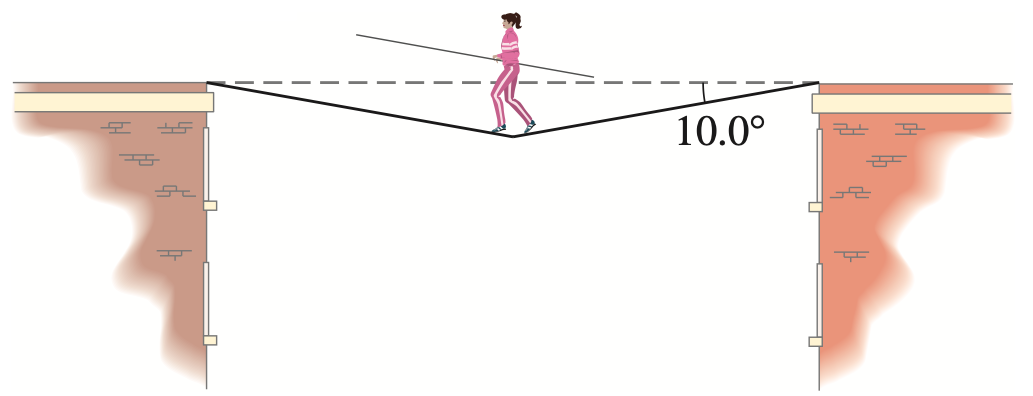
\includegraphics[scale = 0.4]{images/lina.png}
\end{figure}

\begin{minipage}{\linewidth}
\begin{wrapfigure}{r}{0.7in}
\vspace{-4cm}
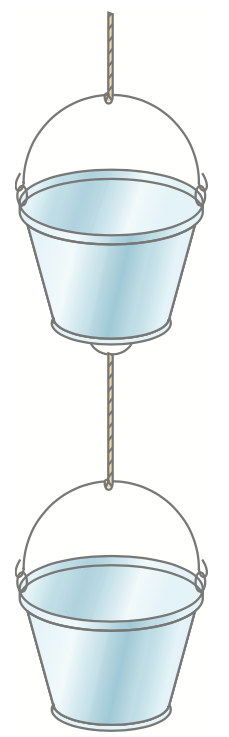
\includegraphics[width=0.7in]{images/fotur.png}
\end{wrapfigure}

\item Málningarfata með massa $\SI{3.2}{kg}$ hengur í reipi fyrir neðan aðra málningarfötu sem hefur massann $\SI{4.5}{kg}$.
\begin{enumerate}[label = \textbf{(\alph*)}]
    \item Hver er togkrafturinn í hvoru reipi fyrir sig ef föturnar eru kyrrstæðar? 
    \item Nú togum við í efra reipið með krafti $\SI{90}{N}$. Hver er hröðun kerfisins?
\end{enumerate}

\end{minipage}

\vspace{0.4cm}

\begin{minipage}{\linewidth}
\begin{wrapfigure}{r}{1.5in}
\vspace{-0.5cm}
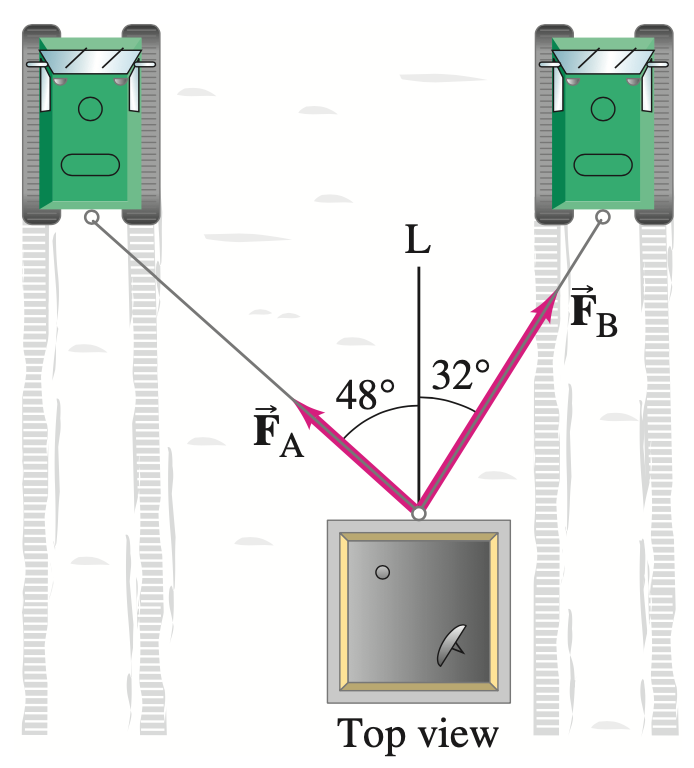
\includegraphics[width=1.5in]{images/snowcat.png}
\end{wrapfigure}

\item Tvær beitidráttarvélar eru að draga litla veðurathuganarstöð á Suðurskautslandinu. Önnur beitidráttarvélin dregur veðurathuganarstöðina með krafti $F_A = \SI{4500}{N}$. Beitidráttarvélarnar draga veðurathuganartöðina þannig að kraftarnir $\vec{F}_A$ og $\vec{F}_B$ mynda hornin $\alpha = \ang{48}$ og $\beta = \ang{32}$ miðað við þá stefnu sem að beitidráttarvélin er að ferðast eftir. Ákvarðið stærð kraftsins $F_B$ og heildarkraftinn $\vec{F} = \vec{F}_A + \vec{F}_B$ sem verkar á veðurathuganarstöðina.
\end{minipage}

\vspace{0.5cm}

\begin{minipage}{\linewidth}
\begin{wrapfigure}{r}{1.5in}
\vspace{0.5cm}
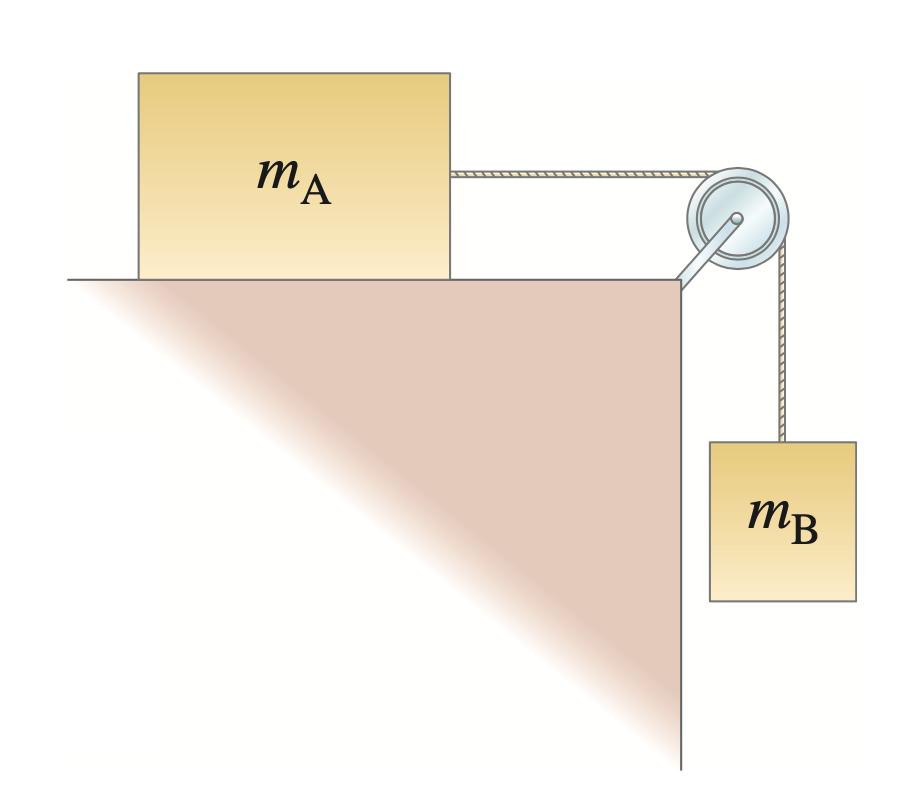
\includegraphics[width=1.5in]{images/trissbert.png}
\end{wrapfigure}

\item Á myndinni hér til hægri má sjá kassa með massa $m_A = \SI{13.0}{kg}$ sem stendur á núningslausu borði í fjarlægð $\SI{1.250}{m}$ frá borðsbrúninni. Kassinn er tengdur með reipi yfir núningslausa trissu við kassa með massa $m_B = \SI{5.0}{kg}$ sem hangir fram af borðinu.
\begin{enumerate}[label = \textbf{(\alph*)}]
    \item Teiknið kraftamynd af hvorum kassa fyrir sig.
    \item Ákvarðið heildarhröðun kerfisins og togkraftinn í reipinu.
    \item Hversu langur tími líður þar til að $m_A$ flýgur fram af borðsbrúninni ef hann er kyrrstæður til að byrja með?
    \item Breytum núna massanum $m_B = \SI{1.0}{kg}$. Hversu stór þyrfti $m_A$ að vera til þess að hröðun kerfisins væri $\frac{1}{100}g = \SI{0.0982}{m/s^2}$?
\end{enumerate}

\end{minipage}

\begin{minipage}{\linewidth}
\begin{wrapfigure}{r}{1.7in}
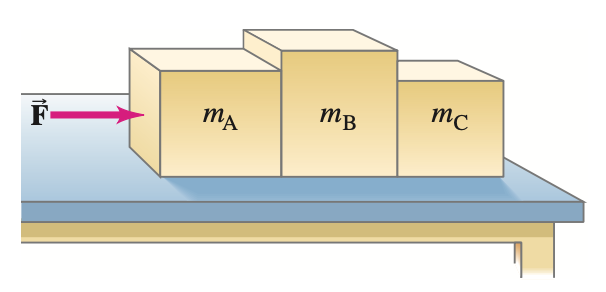
\includegraphics[width=2in]{images/3kubbar.png}
\end{wrapfigure}

\item Þrír kassar, $A,B$ og $C$ með massa $m_A = \SI{8.1}{kg}$, $m_B = \SI{9.7}{kg}$ og $m_C = \SI{8.5}{kg}$ standa á núningslausum fleti. Krafti $F = \SI{96.0}{N}$ er beitt á kassa $A$.
\begin{enumerate}[label = \textbf{(\alph*)}]
    \item Teiknið kraftamyndir af hverjum kubb fyrir sig.
    \item Ákvarðið hröðun kerfisins.
    \item Ákvarðið heildarkraftinn sem verkar á hvern kubb.
    \item Ákvarðið kraftinn $\vec{F}_{B \to A}$ sem kassi $B$ verkar með á $A$.
    \item Ákvarðið kraftinn $\vec{F}_{A \to B}$ sem kassi $A$ verkar með á $B$.
    \item Ákvarðið kraftana $\vec{F}_{B \to C}$ og $\vec{F}_{C \to B}$ sem kassi $B$ og $C$ verka með á hvorn annan.
\end{enumerate}

\end{minipage}

\vspace{0.3cm}

\begin{minipage}{\linewidth}
\begin{wrapfigure}{r}{1.5in}
\vspace{-3.5cm}
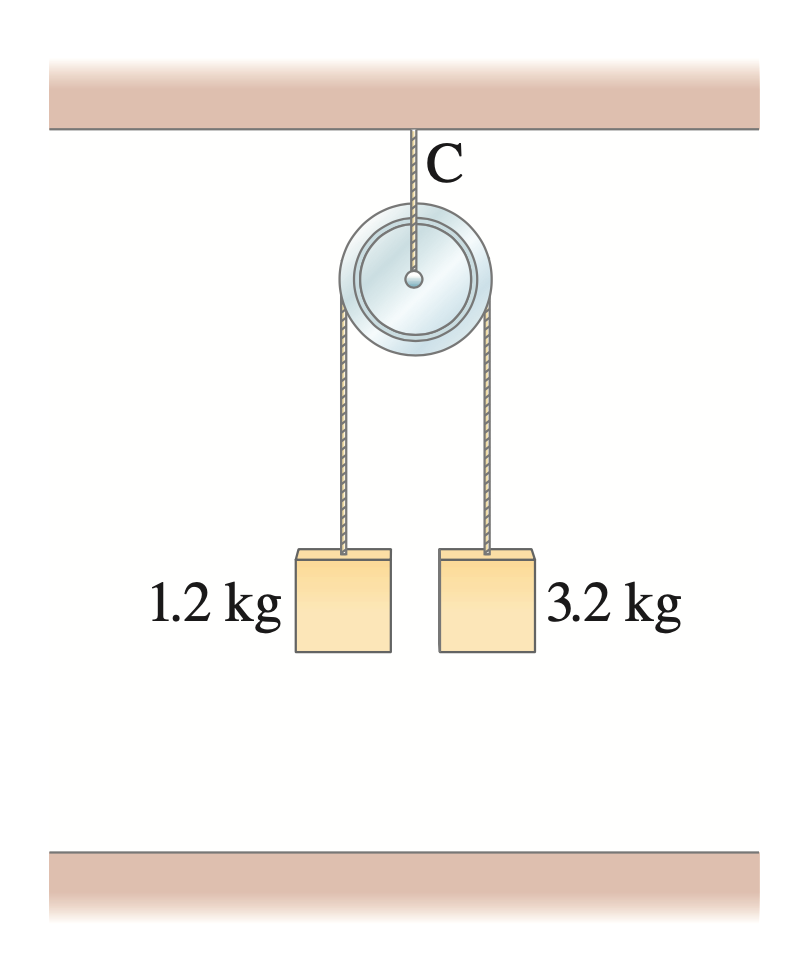
\includegraphics[width=1.5in]{images/atwood.png}
\end{wrapfigure}

\item Lítum á Atwood vélina á mynd hér til hægri. Tveir massar $m_1 = \SI{1.2}{kg}$ og $m_2 = \SI{3.2}{kg}$ eru tengdir saman yfir núningslausa trissu. Ákvarðið togkraftinn í reipinu eftir að mössunum er sleppt úr kyrrstöðu.

\item Núningsstuðullinn milli $\SI{22}{kg}$ kassa og gólfsins er $\mu = \SI{0.30}{}$. Hversu stóran láréttan kraft þarf til þess að draga kassann með jöfnum hraða meðfram gólfinu?

\end{minipage}

\item Hugsum okkur að við stöndum um borð í lest sem tekur af stað með hröðun $a = \SI{1.95}{m/s^2}$. Hver er minnsti núningsstuðullinn milli lestargólfsins og skósólanna til þess að við rennum ekki til?

\item Núningsstuðullinn milli bíldekkja og malbiks er $\mu = \SI{0.90}{}$. Hvert er stærsta hornið miðað við lárétt sem hægt er að leggja bíl í brekku við án þess að hann renni niður brekkuna?

\item Kassa er ýtt af stað með upphafshraða $v_0 = \SI{3.5}{m/s}$. Hversu langt mun kassinn renna ef núningsstuðullinn milli gólfsins og kassans er $\mu = \SI{0.15}{}$.

\begin{minipage}{\linewidth}
\begin{wrapfigure}{r}{1.5in}
\vspace{-0.75cm}
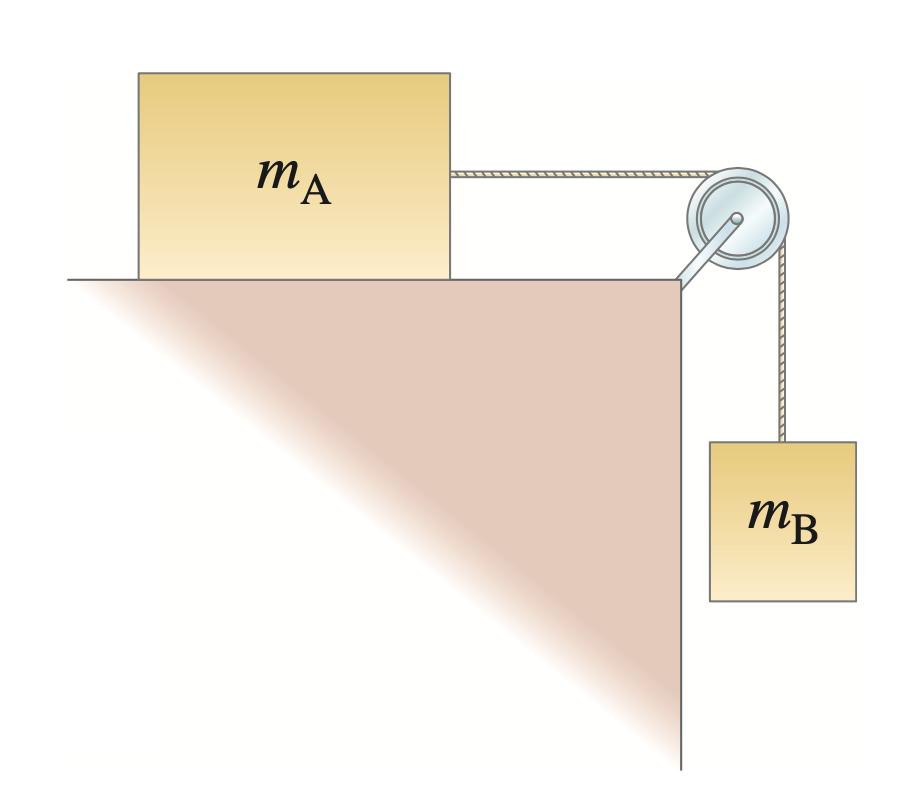
\includegraphics[width=1.5in]{images/trissbert.png}
\end{wrapfigure}

\item Á mynd hér til hægri má sjá kassa með massa $m_A$ sem stendur á borði í fjarlægð $\SI{1.250}{m}$ frá borðsbrúninni. Núningsstuðullinn milli kassans og borðsins er $\mu = \SI{0.20}{}$. Kassinn er tengdur með reipi yfir núningslausa trissu við kassa með massa $m_B = \SI{2.0}{kg}$ sem hangir fram af borðinu. Hvert er minnsta gildið á massanum $m_A$ þannig að kerfið haldist kyrrt?

\end{minipage}

\vspace{0.3cm}

\begin{minipage}{\linewidth}
\begin{wrapfigure}{r}{1.5in}
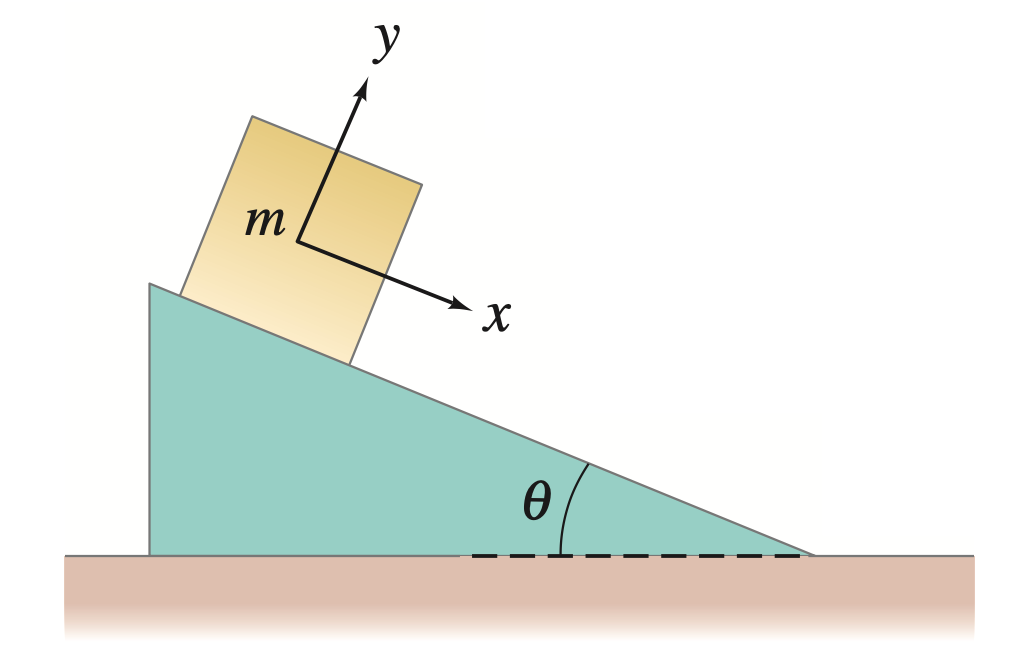
\includegraphics[width=1.5in]{images/skabr2.png}
\end{wrapfigure}

\item Kassi með massa $m = \SI{7.0}{kg}$ hvílir á núningslausu skábretti sem hallar um $\theta = \ang{22.0}$ miðað við lárétt.
\begin{enumerate}[label = \textbf{(\alph*)}]
    \item Ákvarðið hröðun kassans þegar hann rennur niður skábrettið.
    \item Ef kassinn byrjar í hæð $h = \SI{12.0}{m}$ hver verður hraði hans þegar hann kemur niður á botn skábrettisins?
    \item Er heildarorka kassans varðveitt við að renna niður skábrettið?
\end{enumerate}

\end{minipage}

\item Kassi fær upphafshraða $v_0 = \SI{4.5}{m/s}$ upp núningslaust skábretti sem hallar um $\theta = \ang{22.0}$ miðað við lárétt.
\begin{enumerate}[label = \textbf{(\alph*)}]
    \item Hversu hátt kemst kubburinn áður en hann stoppar í efstu hæð?
    \item Hversu langur tími líður þar til að hann er í efstu hæð?
    \item Hversu langur tími líður þar til að hann er búinn að renna aftur niður skábrettið?
\end{enumerate}

\item Skoðum núna kubb með massa $m$ sem stendur á skábretti sem hallar um $\theta = \ang{25.0}$ miðað við lárétt. Látum núningsstuðulinn milli kassans og undirlagsins vera $\mu = \SI{0.19}{}$.
\begin{enumerate}[label = \textbf{(\alph*)}]
    \item Ákvarðið hröðun kubbsins, $a$, á meðan hann rennur niður skábrettið.
    
    \item Ákvarðið hraða kubbsins þegar hann kemur niður skábrettið ef hann byrjar í $h = \SI{8.15}{m}$ hæð.
    
    \item Nú er kubbnum ýtt upp skábrettið með upphafshraða $v_0 = \SI{3.0}{m/s}$. Hversu hátt kemst kubburinn áður en að hann staðnæmist  í efstu stöðu? Hversu langan tíma tók það?
\end{enumerate}


\item Barn rennir sér niður rennibraut sem hallar um $\theta = \ang{34}$ miðað við lárétt. Á botni rennibrautarinnar er hraði barnsins helmingurinn af þeim hraða sem barnið hefði haft ef rennibrautin hefði verið núningslaus. Ákvarðið núningsstuðulinn milli barnsins og rennibrautarinar.

\vspace{0.3cm}

\begin{minipage}{\linewidth}
\begin{wrapfigure}{r}{2.5in}
\vspace{0.5cm}
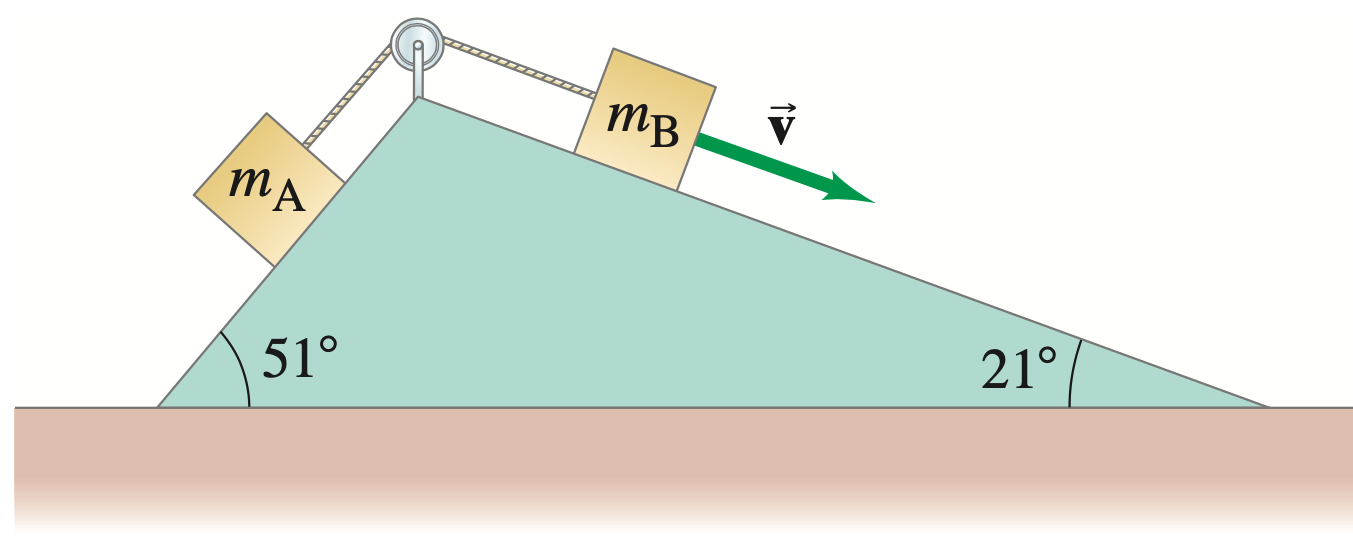
\includegraphics[width=2.5in]{images/skabr4.png}
\end{wrapfigure}

\item Tveir kassar með massa $m_A = \SI{2.0}{kg}$ og $m_B = \SI{5.0}{kg}$ standa á undarlegu skábretti (sjá mynd hér til hægri). Kassarnir eru tengdir með reipi yfir núningslausa trissu. Flöturinn sem $m_A$ hvílir á hallar um $\alpha = \ang{51}$ miðað við lárétt en flöturinn sem $m_B$ hvílir á hallar um $\beta = \ang{21}$ miðað við lárétt. Núningsstuðullinn milli $m_A$ og flatarins sem hann hvílir á er $\mu_A = \SI{0.25}{}$ en núningsstuðullinn milli $m_B$ og flatarins sem hann hvílir á er $\mu_B = \SI{0.30}{}$. Ákvarðið hröðun kerfisins að því gefnu að $m_A$ færist upp skábrettið sitt en $m_B$ færist niður skábrettið sitt.
\end{minipage}

\vspace{0.3cm}

\begin{minipage}{\linewidth}
\begin{wrapfigure}{r}{2.5in}
\vspace{-1cm}
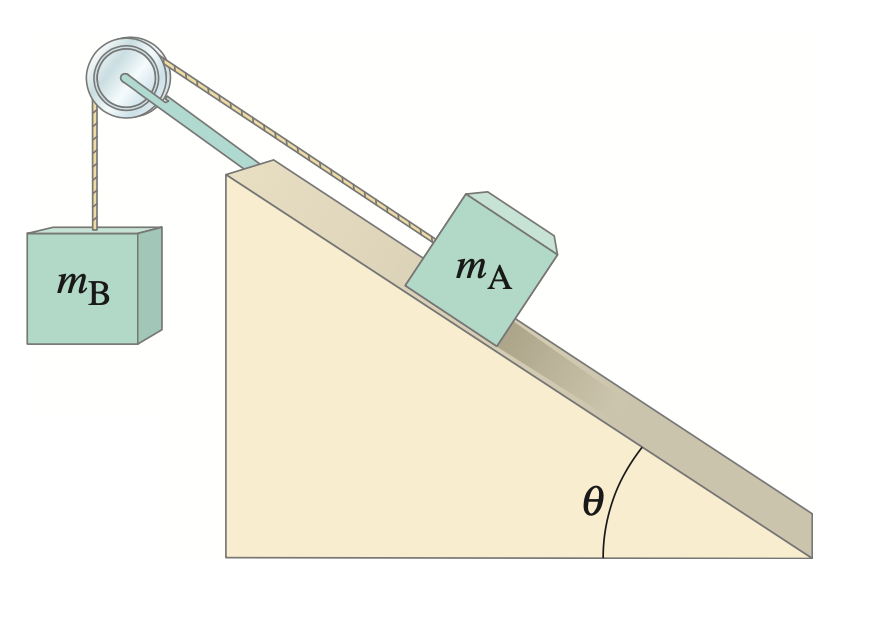
\includegraphics[width=2.5in]{images/hanger.png}
\end{wrapfigure}

\item Skoðum myndina hér til hægri. Tveir kassar með massa $m_A = \SI{2.7}{kg}$ og $m_B = \SI{3.2}{kg}$ eru tengdir með reipi yfir núningslausa trissu. Kassinn með massa $m_A$ hvílir á skábretti sem hallar um $\theta = \ang{34}$ miðað við lárétt.  Núningsstuðullinn milli $m_A$ og skábrettisins er $\mu = \SI{0.15}{}$. \textbf{(a)} Ákvarðið hröðun kerfisins þegar því er sleppt úr kyrrstöðu að því gefnu að $m_B$ byrjar að færist niður (og $m_A$ þar af leiðandi upp, samsíða skábrettinu).  \textbf{(b)} Hvert er minnsta gildið á $\mu$ þannig að kerfið haldist kyrrt?

\end{minipage}

\vspace{0.3cm}

\begin{minipage}{\linewidth}
\begin{wrapfigure}{r}{1.5in}
\vspace{-0.5cm}
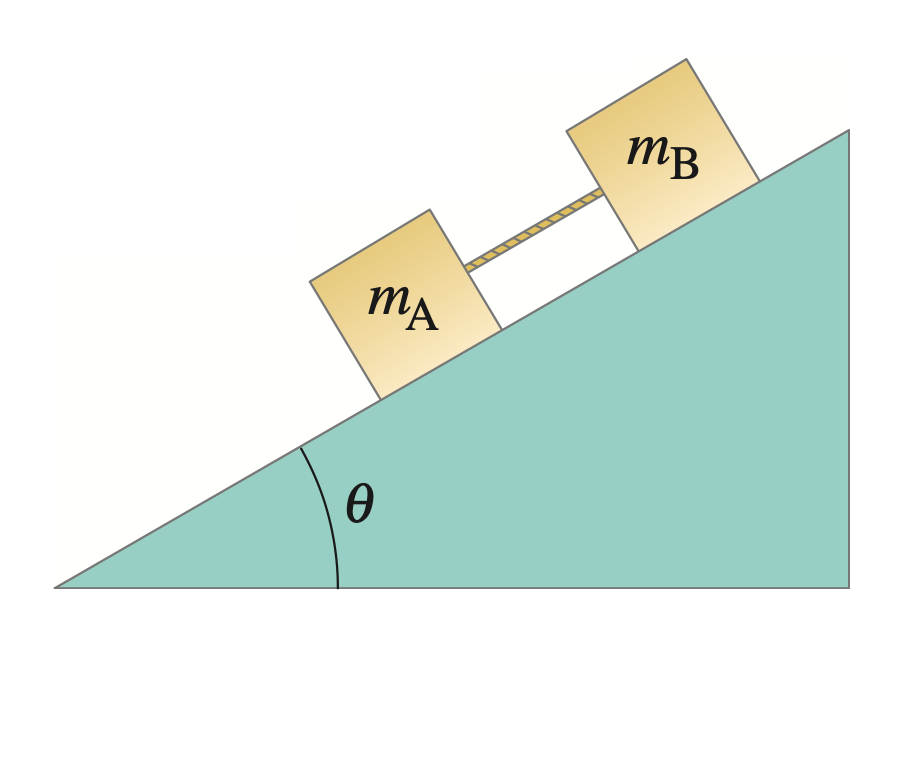
\includegraphics[width=1.5in]{images/skabr3.png}
\end{wrapfigure}

\item Tveir kassar með massa $m_A = \SI{5.0}{kg}$ og $m_B = \SI{4.2}{kg}$ eru tengdir með reipi og standa á skábretti sem hallar um $\theta = \ang{32}$ gráður miðað við lárétt. Kassarnir eru úr mismunandi efnum svo að núningsstuðullinn milli kassa $A$ og skábrettisins er $\mu_A = \SI{0.20}{}$ en núningsstuðullinn milli kassa $B$ og skábrettisins er $\mu_B$. Ákvarðið hröðun kerfisins og togkraftinn í reipinu.
\end{minipage}

\newpage

\subsection*{Gömul prófdæmi}


\item Tveir massar $m_1 = \SI{1.0}{kg}$ og $m_2 = \SI{2.0}{kg}$ liggja á núningslausum, láréttum fleti. Þeir eru festir saman með vír og eru togaðir af öðrum vír sem er festur við massann $m_3 = \SI{3.0}{kg}$ sem hangir undir massalausri, núningslausri trissu. Gera má ráð fyrir að vírarnir séu massalausir.
\begin{enumerate}[label = \textbf{(\alph*)}]
    \item Merkið inn á myndina kraftana sem verka á hvern massa fyrir sig.
    \item Skrifið niður kraftajöfnur fyrir alla massana.
    \item Finnið heildarhröðun kerfisins, $a$.
    \item Finnið togkraftinn, $T_2$, í vírnum sem tengir saman massana $m_2$ og $m_3$.
\end{enumerate}

\begin{center}
\begin{tikzpicture}[every node/.style={minimum size=0.9cm}]
           \draw [line width = 0.6 pt] (0,-3) -- (0,0); 
           \draw [line width = 0.6pt] (0,0) -- (6.2,0); 
           \node [line width = 0.4pt, draw] at (2.0,0.45) {\(m_2\)}; 
           \node [line width = 0.4pt, draw] at (4.4,0.45) {\(m_1\)};
           \node [line width = 0.8pt] at (-0.8,-2) { \(m_3\)}; 
           \draw (-1.2,-2.5) -- (-1.2,-1.5) -- (-0.4,-1.5) -- (-0.4,-2.5) -- (-1.2,-2.5); //Massi 3
           \draw (-0.6,0.4) circle (0.25 cm);
           \draw [line width = 0.4pt, draw] (0,0) -- (-0.38, 0.3); 
           \draw (-0.6,0.4) circle (0.25 cm);
           \fill[black] (-0.6,0.4) circle (0.05 cm);
           \draw [line width = 0.4pt, draw] (-0.6,0.65) -- (1.55, 0.65);
           \draw [line width = 0.4pt, draw] (2.45,0.65) -- (3.95, 0.65);
           \draw [line width = 0.4 pt] (-0.86,0.4) -- (-0.86,-1.5);
           \node  at (3.2, 1.1) { \(T_1\)};
           \node  at (0.5, 1.1) { \(T_2\)};
   \end{tikzpicture}
\end{center}

\item Kubbur með massa $m_1 = \SI{10}{kg}$ stendur kyrr á skábretti sem hallar um hornið $\theta = \ang{27}$. Kubburinn er festur yfir trissu við vatnsfötu með massa $m_2 = \SI{5.0}{kg}$. Gerum ráð fyrir að hlutfallið $\frac{m_1}{m_2}$ og hornið $\theta$ séu þannig að kassinn byrji að renna úr kyrrstöðu. Núningsstuðullinn milli kubbsins með massa $m_1$ og skábrettisins er $\mu = 0.20$.
\begin{enumerate}[label = \textbf{(\alph*)}]
    \item Gerið kraftamynd og skrifið niður kraftajöfnur fyrir báða massana.
    
    \item Finnið hröðun kubbsins í stefnu samsíða skábrettinu.
    \item  Finnið tímann $t$ sem það tekur kubbinn að renna niður skábrettið um vegalengd $s$.
    \item Kubbnum með massa $m_1$ er aftur komið fyrir í upphafsstöðu og er haldið kyrrum meðan vatni er hellt ofan í fötuna. Hversu miklu vatni, $m_{\text{vatn}}$, þarf að hella ofan í fötuna svo að $m_1$ verði kyrr á skábrettinu eftir að honum er sleppt?
\end{enumerate}

\begin{figure}[H]
    \centering
    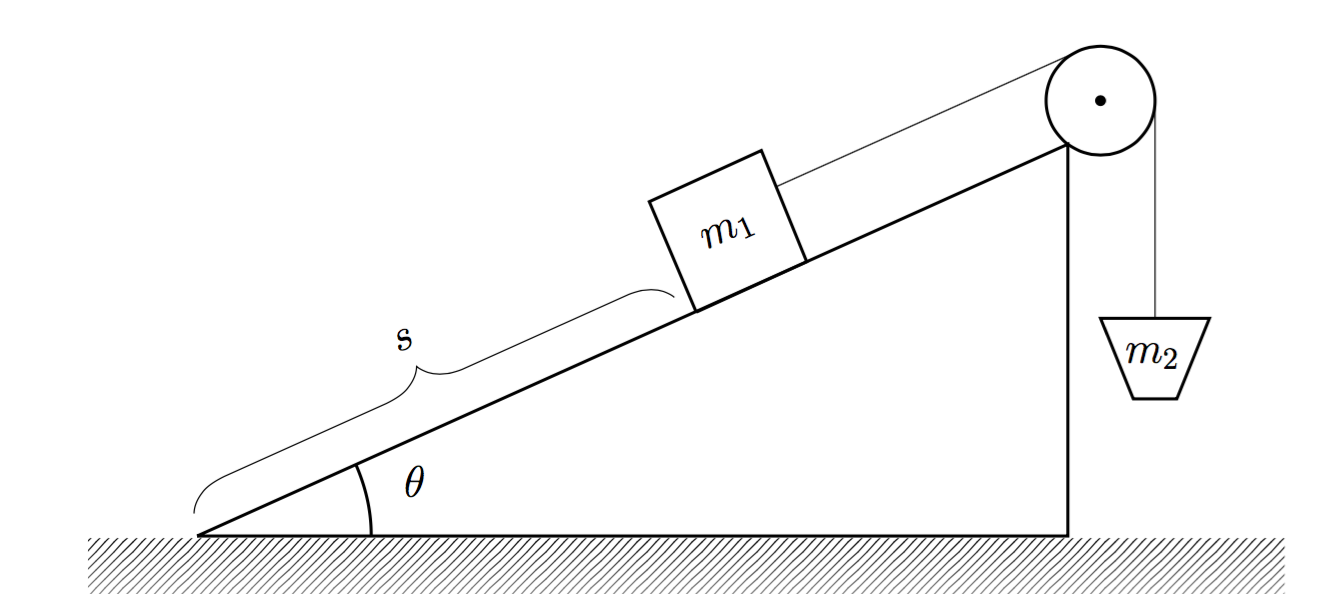
\includegraphics[scale = 0.5]{images/vatnsfata.png}
\end{figure}

\begin{minipage}{\linewidth}
\begin{wrapfigure}{r}{2in}
\vspace{-0.5cm}
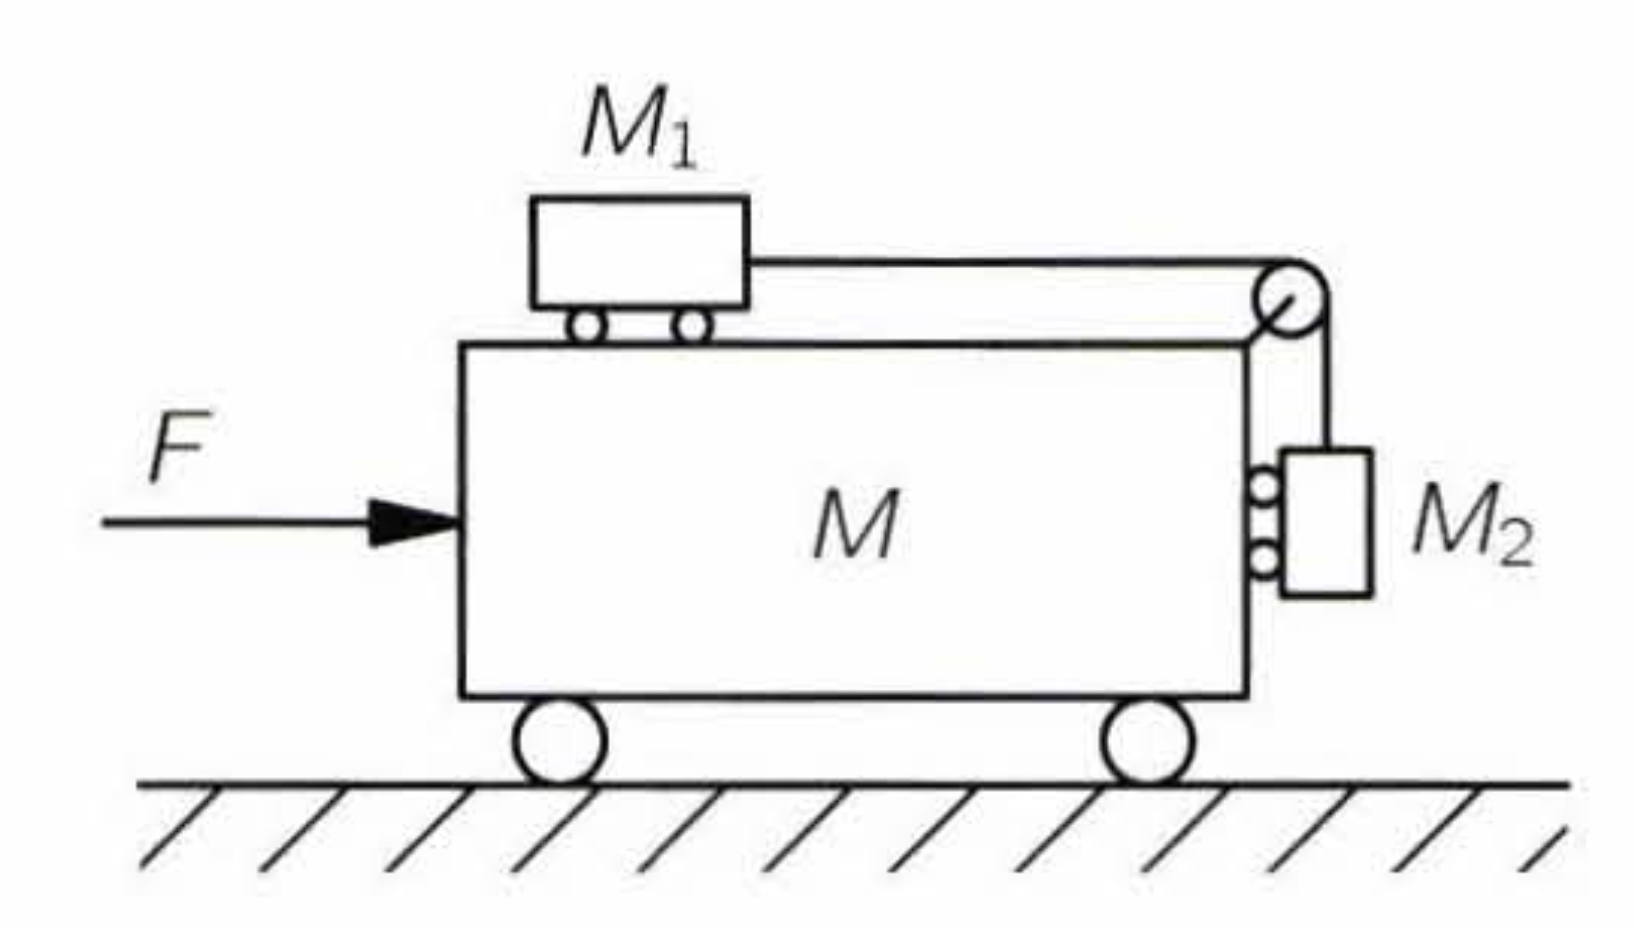
\includegraphics[width=2in]{images/feyn.png}
\end{wrapfigure}


\item Finnið lárétta kraftinn $F$ sem þarf til þess að $M_1$ og $M_2$ haldist kyrrir miðað við $M$. Hunsið áhrif núningskraftsins.

\end{minipage}

\newpage

\begin{minipage}{\linewidth}
\begin{wrapfigure}{r}{1.5in}
\vspace{-1cm}
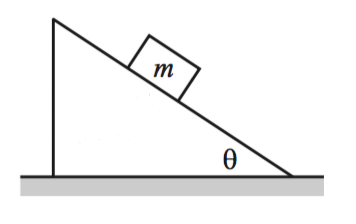
\includegraphics[width=1.5in]{images/skasson.png}
\end{wrapfigure}

\item Kubbur með massa $m = \SI{13}{kg}$ ferðast upp skáplan með upphafshraðanum $v_0 = \SI{6.0}{m/s}$. Skáplanið hallar um $\theta = \SI{25}{\degree}$ miðað við lárétt. Kubburinn kemst í mestu hæð $\SI{0,80}{m}$ áður en hann stöðvast. Finnið hreyfinúningsstuðulinn, $\mu$, milli kubbsins og skáplansins.
\end{minipage}

\item Bergljót er að færa stóra, þunga eldavél með massa $m = \SI{120}{kg}$ í íbúðinni sinni. Núningsstuðullinn milli eldavélarinnar og gólfsins er $\mu = 0,40$. Bergljót þarf að draga eldavélina með jöfnum hraða svo hún springi ekki. Finnið með hversu stórum krafti, $F$, Bergljót þarf að draga eldavélina svo hún springi ekki, ef hún togar undir gefnu horni $\theta = \SI{31}{\degree}$.

\begin{figure}[H]
    \centering
    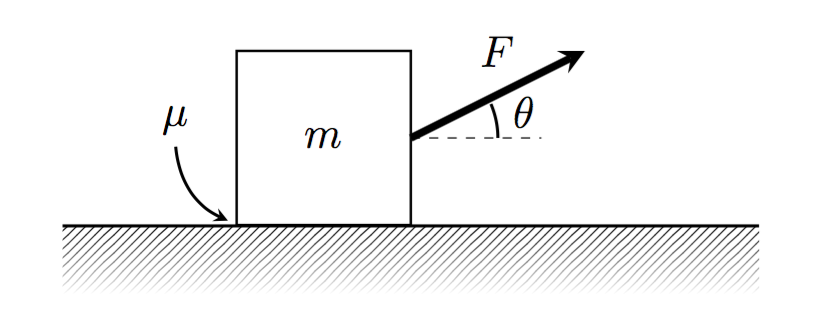
\includegraphics[scale = 0.5]{images/kommoda.png}
\end{figure}

\vspace{-0.5cm}

\item Skábretti með massa $M$, sem hallar um $\alpha$ gráður, stendur kyrrt á núningslausum láréttum fleti. Kassa með massa $m$ er komið fyrir á skábrettinu, samtímis er láréttum krafti $\Vec{F}$ beitt á skábrettið. Gerum ráð fyrir að enginn núningur verki milli kassans og skábrettisins. Hversu miklum krafti $\Vec{F}$ þarf að beita til þess að kassinn með massa $m$ haldist í fastri hæð?

\begin{figure}[H]
    \centering
    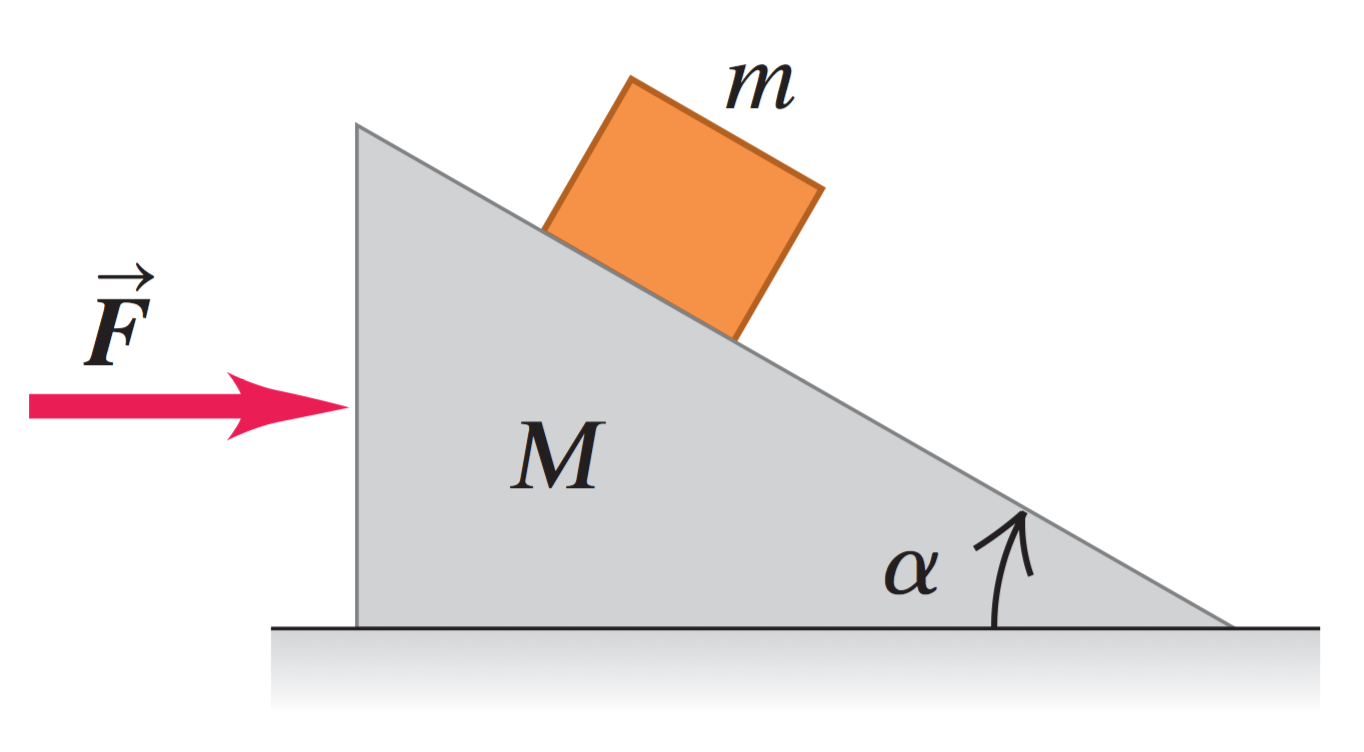
\includegraphics[scale = 0.3]{images/martrod.png}
\end{figure}

\begin{minipage}{\linewidth}
\begin{wrapfigure}{r}{1.5in}
\vspace{-2cm}
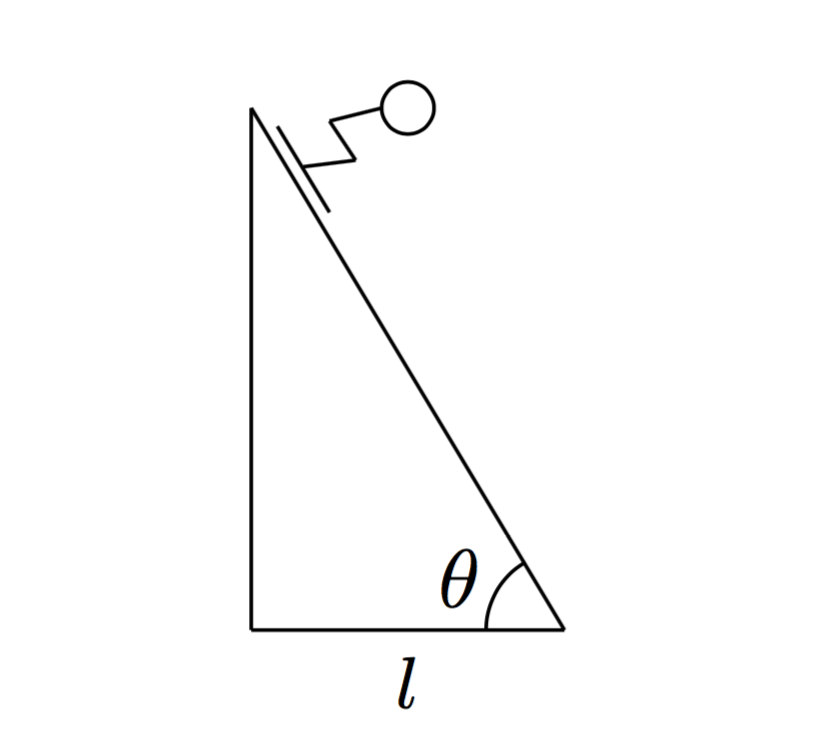
\includegraphics[width=1.5in]{images/skidi.png}
\end{wrapfigure}

\vspace{-0.5cm}

\item Sigbert skíðagarpur rennir sér niður Kóngsbrekkuna í Bláfjöllum sem hefur hallann $\theta = \SI{60}{\degree}$. Núningsstuðullinn milli skíðanna og brekkunnar er $\mu = 0.25$. Skíðagarpurinn vegur $m = \SI{60}{kg}$. Hver verður lokahraði skíðagarpsins ef hann byrjar í toppi brekkunnar og lárétt lengd brekkunnar er $l = \SI{15}{\metre}$.
\end{minipage}

\vspace{0.3cm}

\begin{minipage}{\linewidth}
\begin{wrapfigure}{r}{1.5in}
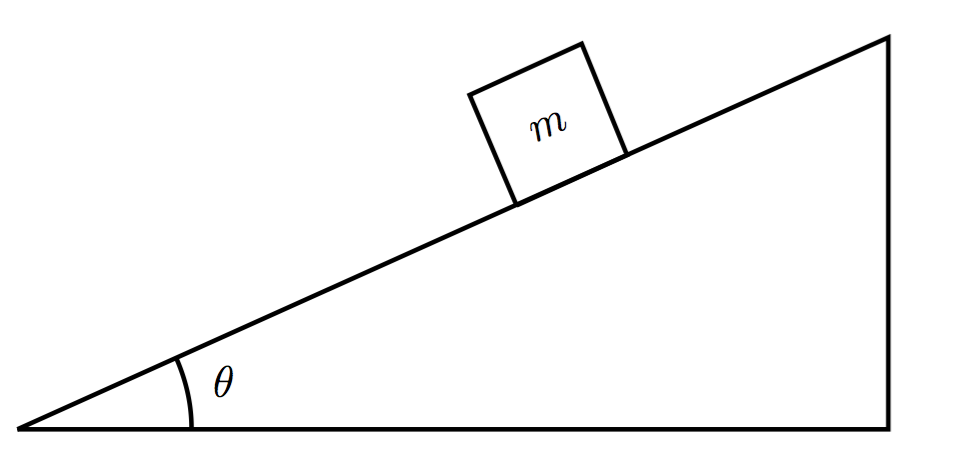
\includegraphics[width=2in]{images/skabjol.png}
\end{wrapfigure}

\item Skíðagarpur með massa $\SI{76}{kg}$ rennir sér niður Skálabrekkuna á Böggvisstaðafjalli. Brekkan er $\SI{310}{m}$ löng og hallar um  $\theta = \ang{22}$ miðað við lárétt. Núningsstuðullinn milli snjós og skíða er $\mu = \SI{0.27}{}$. 
\end{minipage}
\vspace{0.1cm}
\begin{enumerate}[label = \textbf{(\alph*)}]
    \item Gerið kraftamynd af skíðagarpinum og skrifið niður kraftajöfnu.
    \item Hver er hröðun skíðagarpsins niður brekkuna?
    \item Finnið hraða skíðagarpsins þegar hann er kominn niður brekkuna.
    \item Hversu mikil orka tapaðist í núning á leiðinni niður brekkuna?
\end{enumerate}

\begin{minipage}{\linewidth}
\begin{wrapfigure}{r}{1.3in}
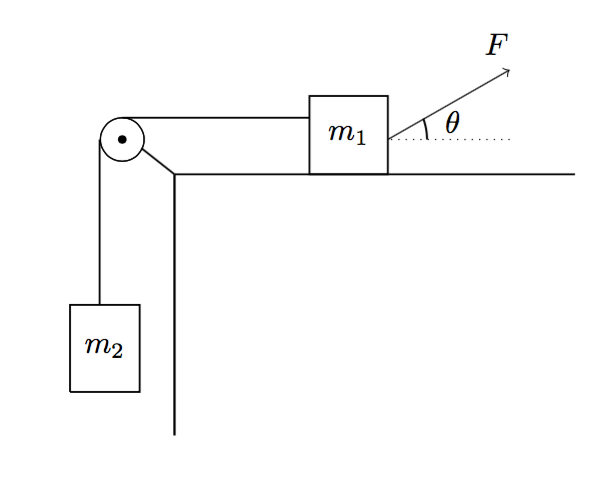
\includegraphics[width=1.8 in]{images/krafta.png}
\end{wrapfigure}

\item Kubbur með massa $m_1 = \SI{5.0}{kg}$ liggur á borði. Hann er festur með massalausu bandi við kubb með massa $m_2 = \SI{3.0}{kg}$ yfir núningslausa, massalausa trissu. Núningsstuðullinn milli borðs og kubbs er $\mu = \SI{0.45}{}$. Leifur ákveður að draga kubbinn á borðinu með krafti $F = \SI{52}{N}$ og horni $\theta = \ang{22}$ miðað við lárétt.

\end{minipage}

\begin{enumerate}[label = \textbf{(\alph*)}]
    \item Teiknið kraftamyndir og skrifið niður kraftajöfnur fyrir báða massana.
    
    \item Finnið þverkraftinn sem verkar á kubbinn á borðinu.
    
    \item Finnið hröðun kerfisins.
    
    \item Finnið togkraftinn í bandinu.
\end{enumerate}

\end{enumerate}
